\chapter{Jenkins}
Bij het ontwikkelen van de verschillende applicaties zal Jenkins gebruikt worden om de verschillende applicaties te bouwen en automatisch te testen aan de hand van unit- en/of integratie tests.

Vanuit docker hub is een image beschikbaar voor Jenkins zodat deze binnen een docker container kan worden uitgevoerd. Deze hebben we dan ook lokaal binnen gehaald door gebruik te maken van Portainer op de docker omgeving.

\begin{figure}[H]
	\centering
	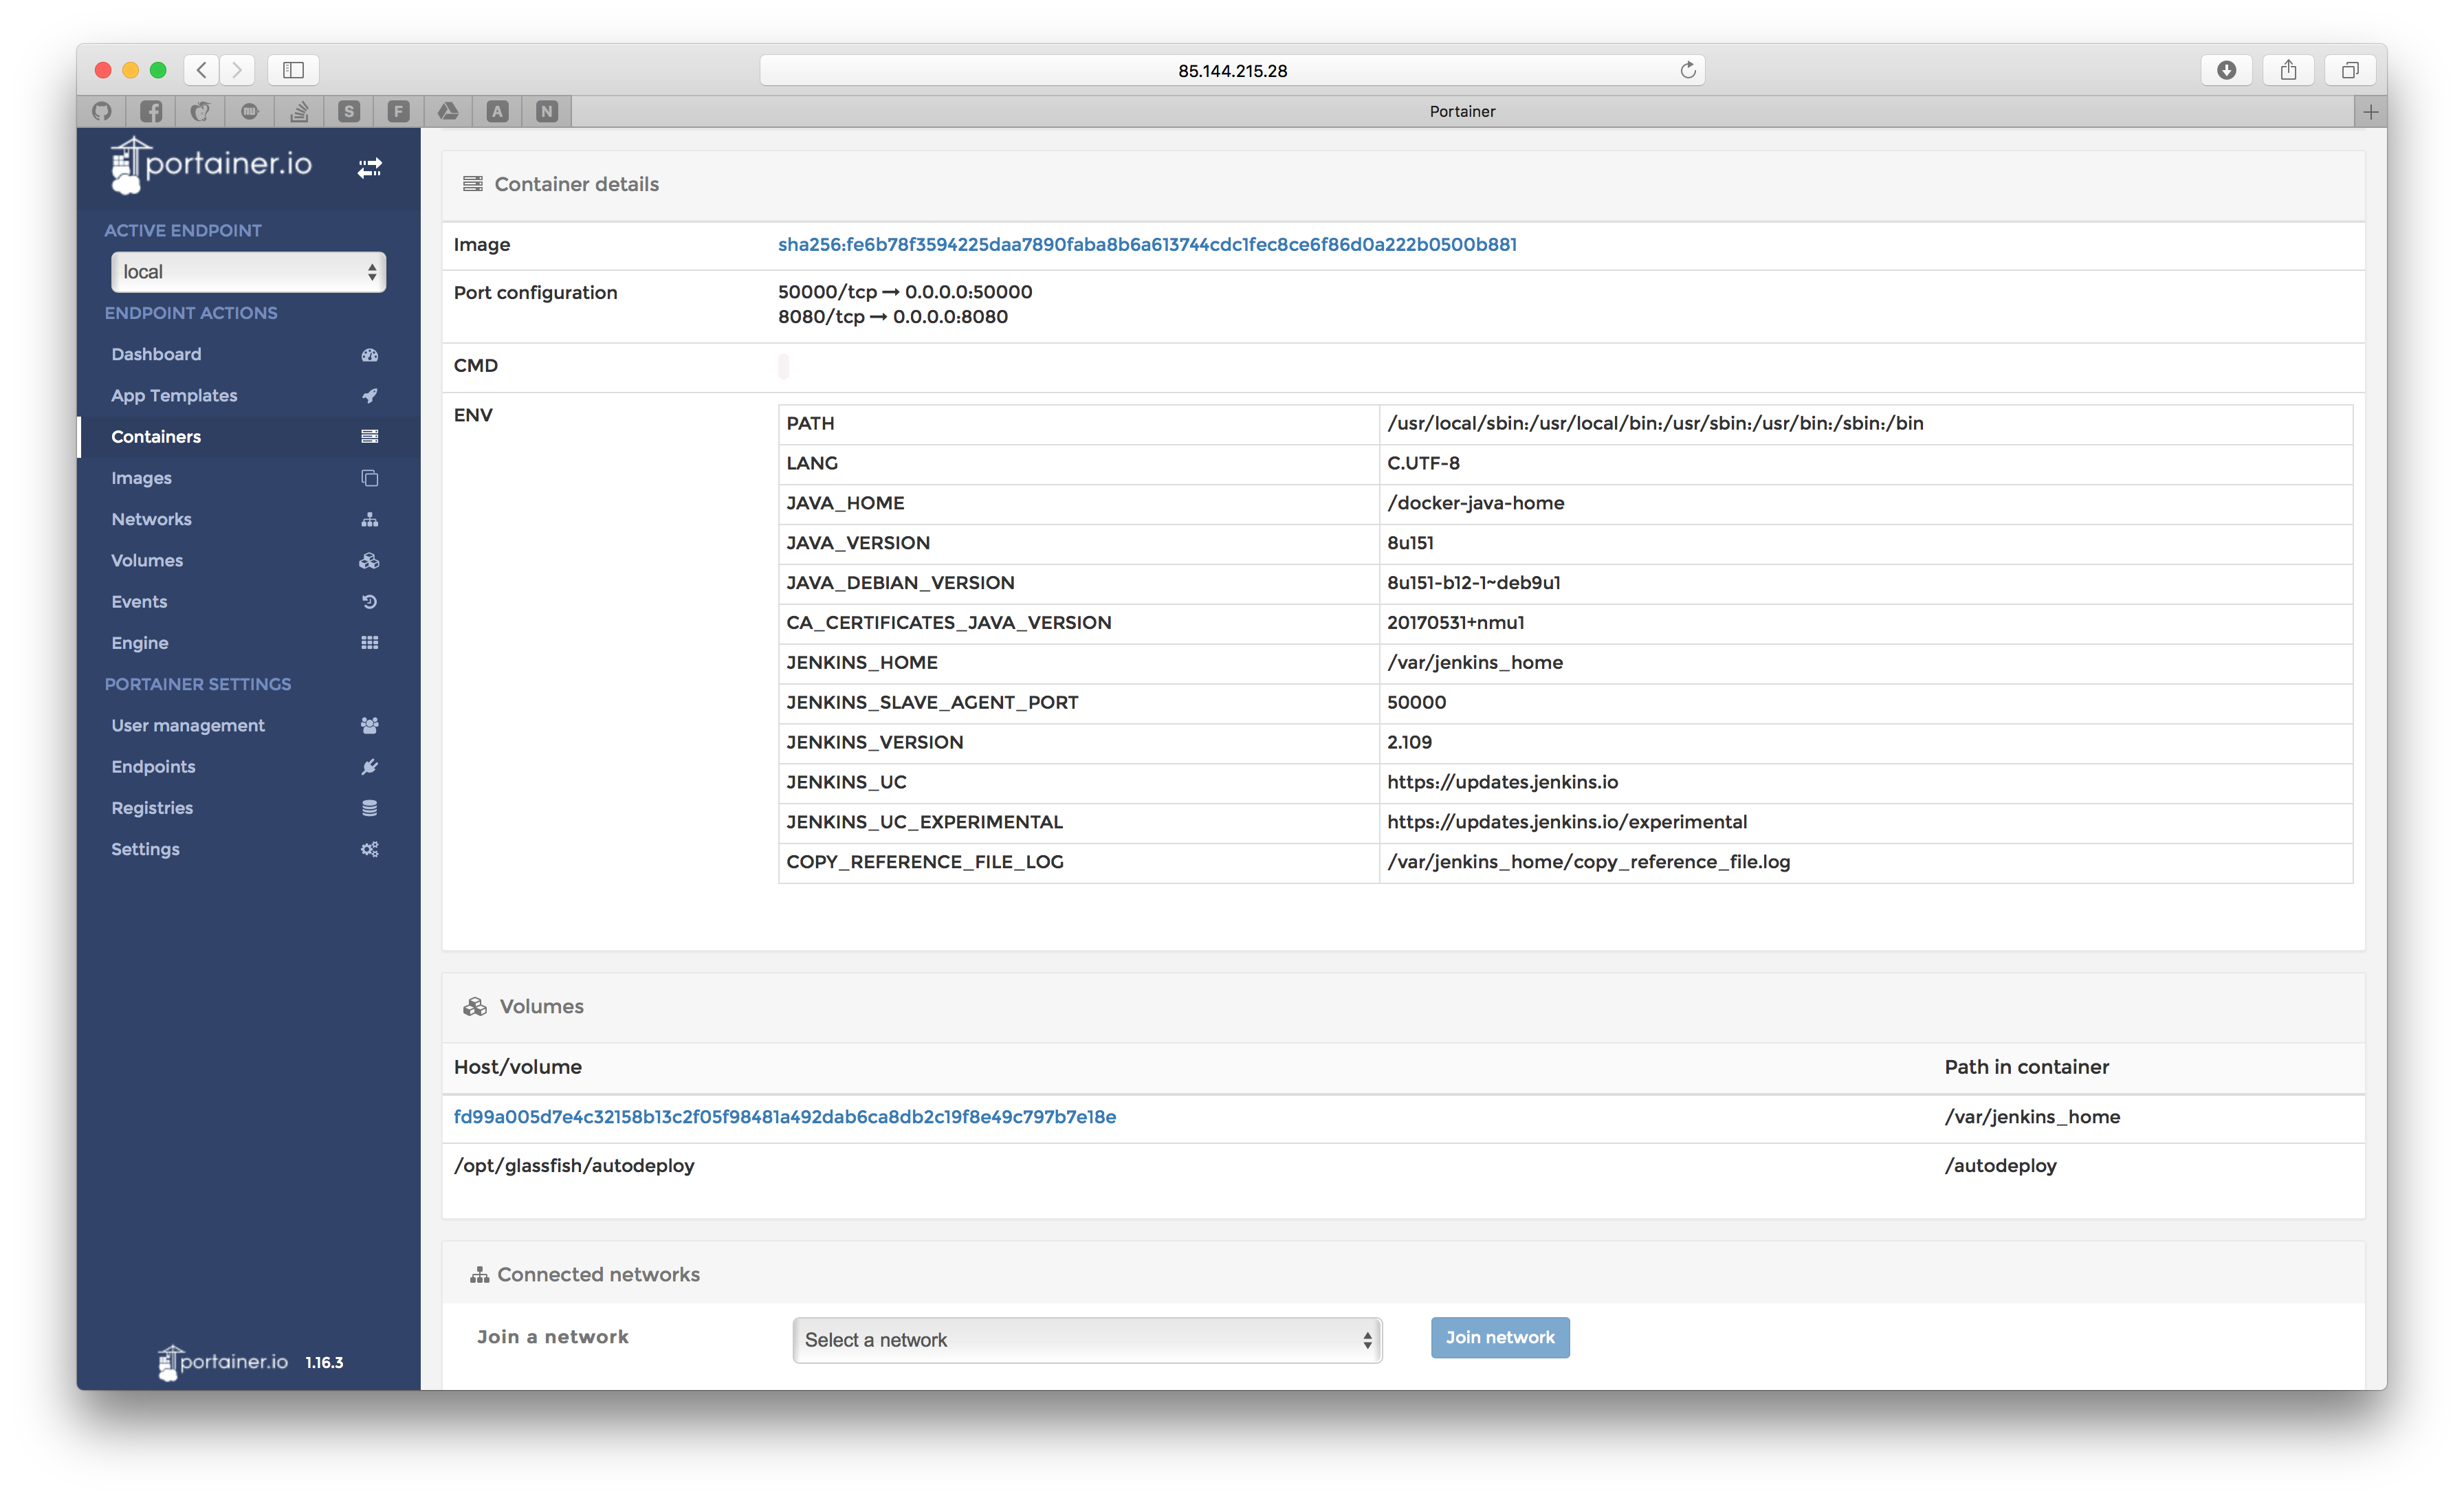
\includegraphics[width=0.95\textwidth]{img/JenkinsContainerDetails.png}
	\caption{Configuratie van port mapping en volume binding voor Jenkins container in docker}
	\label{fig:JenkinsContainerDetails}
\end{figure}

\section{Container Configuratie}
In onderstaande hoofdstukken beschrijven we hoe de Jenkins container geconfigureerd is zodat deze bereikbaar is van buitenaf, maar ook hoe we verschillende applicaties automatisch kunnen deployen op een applicatie server.

\subsection{Port mapping}
Zoals te zien is in figuur \ref{fig:JenkinsContainerDetails} is voor de container waarbinnen Jenkins uitgevoerd zal worden twee verschillende port mappings geconfigureerd, namelijk poort 8080 en 50000.

Poort 8080 wordt gebruikt voor de webinterface. Hierin is het mogelijk om Jenkins te configureren en de voortang van verschillende taken te zien. Poort 50000 wordt gebruikt voor de Java API. Wanneer Jenkins wordt geconfigureerd om te werken met verschillende zoganaamde "slaves" is deze poort vooral belangrijk.

\subsection{Volumes}
Zoals te zien is zijn er twee volumes gekoppeld aan de docker container van Jenkins. Normaliter is dit enkel één volume die de Jenkins Home. Wanneer een build wordt gestart voor een project in Jenkins zal deze worden uitgevoerd in de workspace van het project. Het volledige pad van deze workspace begint met de Jenkins home (/var/jenkins\_home) gevolgd door de naam van het project.

\subsubsection{Autodeploy folder mapping}
//TODO verwijzing naar jenkins project config
Er is voor gekozen om binnen de Jenkins container een extra map de koppelen aan een map op de host machine. Hierdoor kunnen we op een makkelijke manier een nieuwe versie van de applicatie deployen op een applicatie server. De werking van deze autodeploy folder zal in een verder hoofdstuk meer worden uitgelegd.

\section{Configureren van Projecten binnen Jenkins}
Voor alle te ontwikkelen applciaties wordt binnen jenkins een nieuw project aangemaakt. Zoals op Figuur \ref{fig:JenkinsProjectOverview} te zien is, is voor één applicatie meerdere projecten binnen Jenkins beschikbaar. De naamgeving van de verschillende projecten houden we consistent voor alle applicaties door de naam van de applicatie te nemen en vervolgens daarachter de omgeving neer te zetten waar de applicatie is beschikbaar is.

\begin{figure}[H]
	\centering
	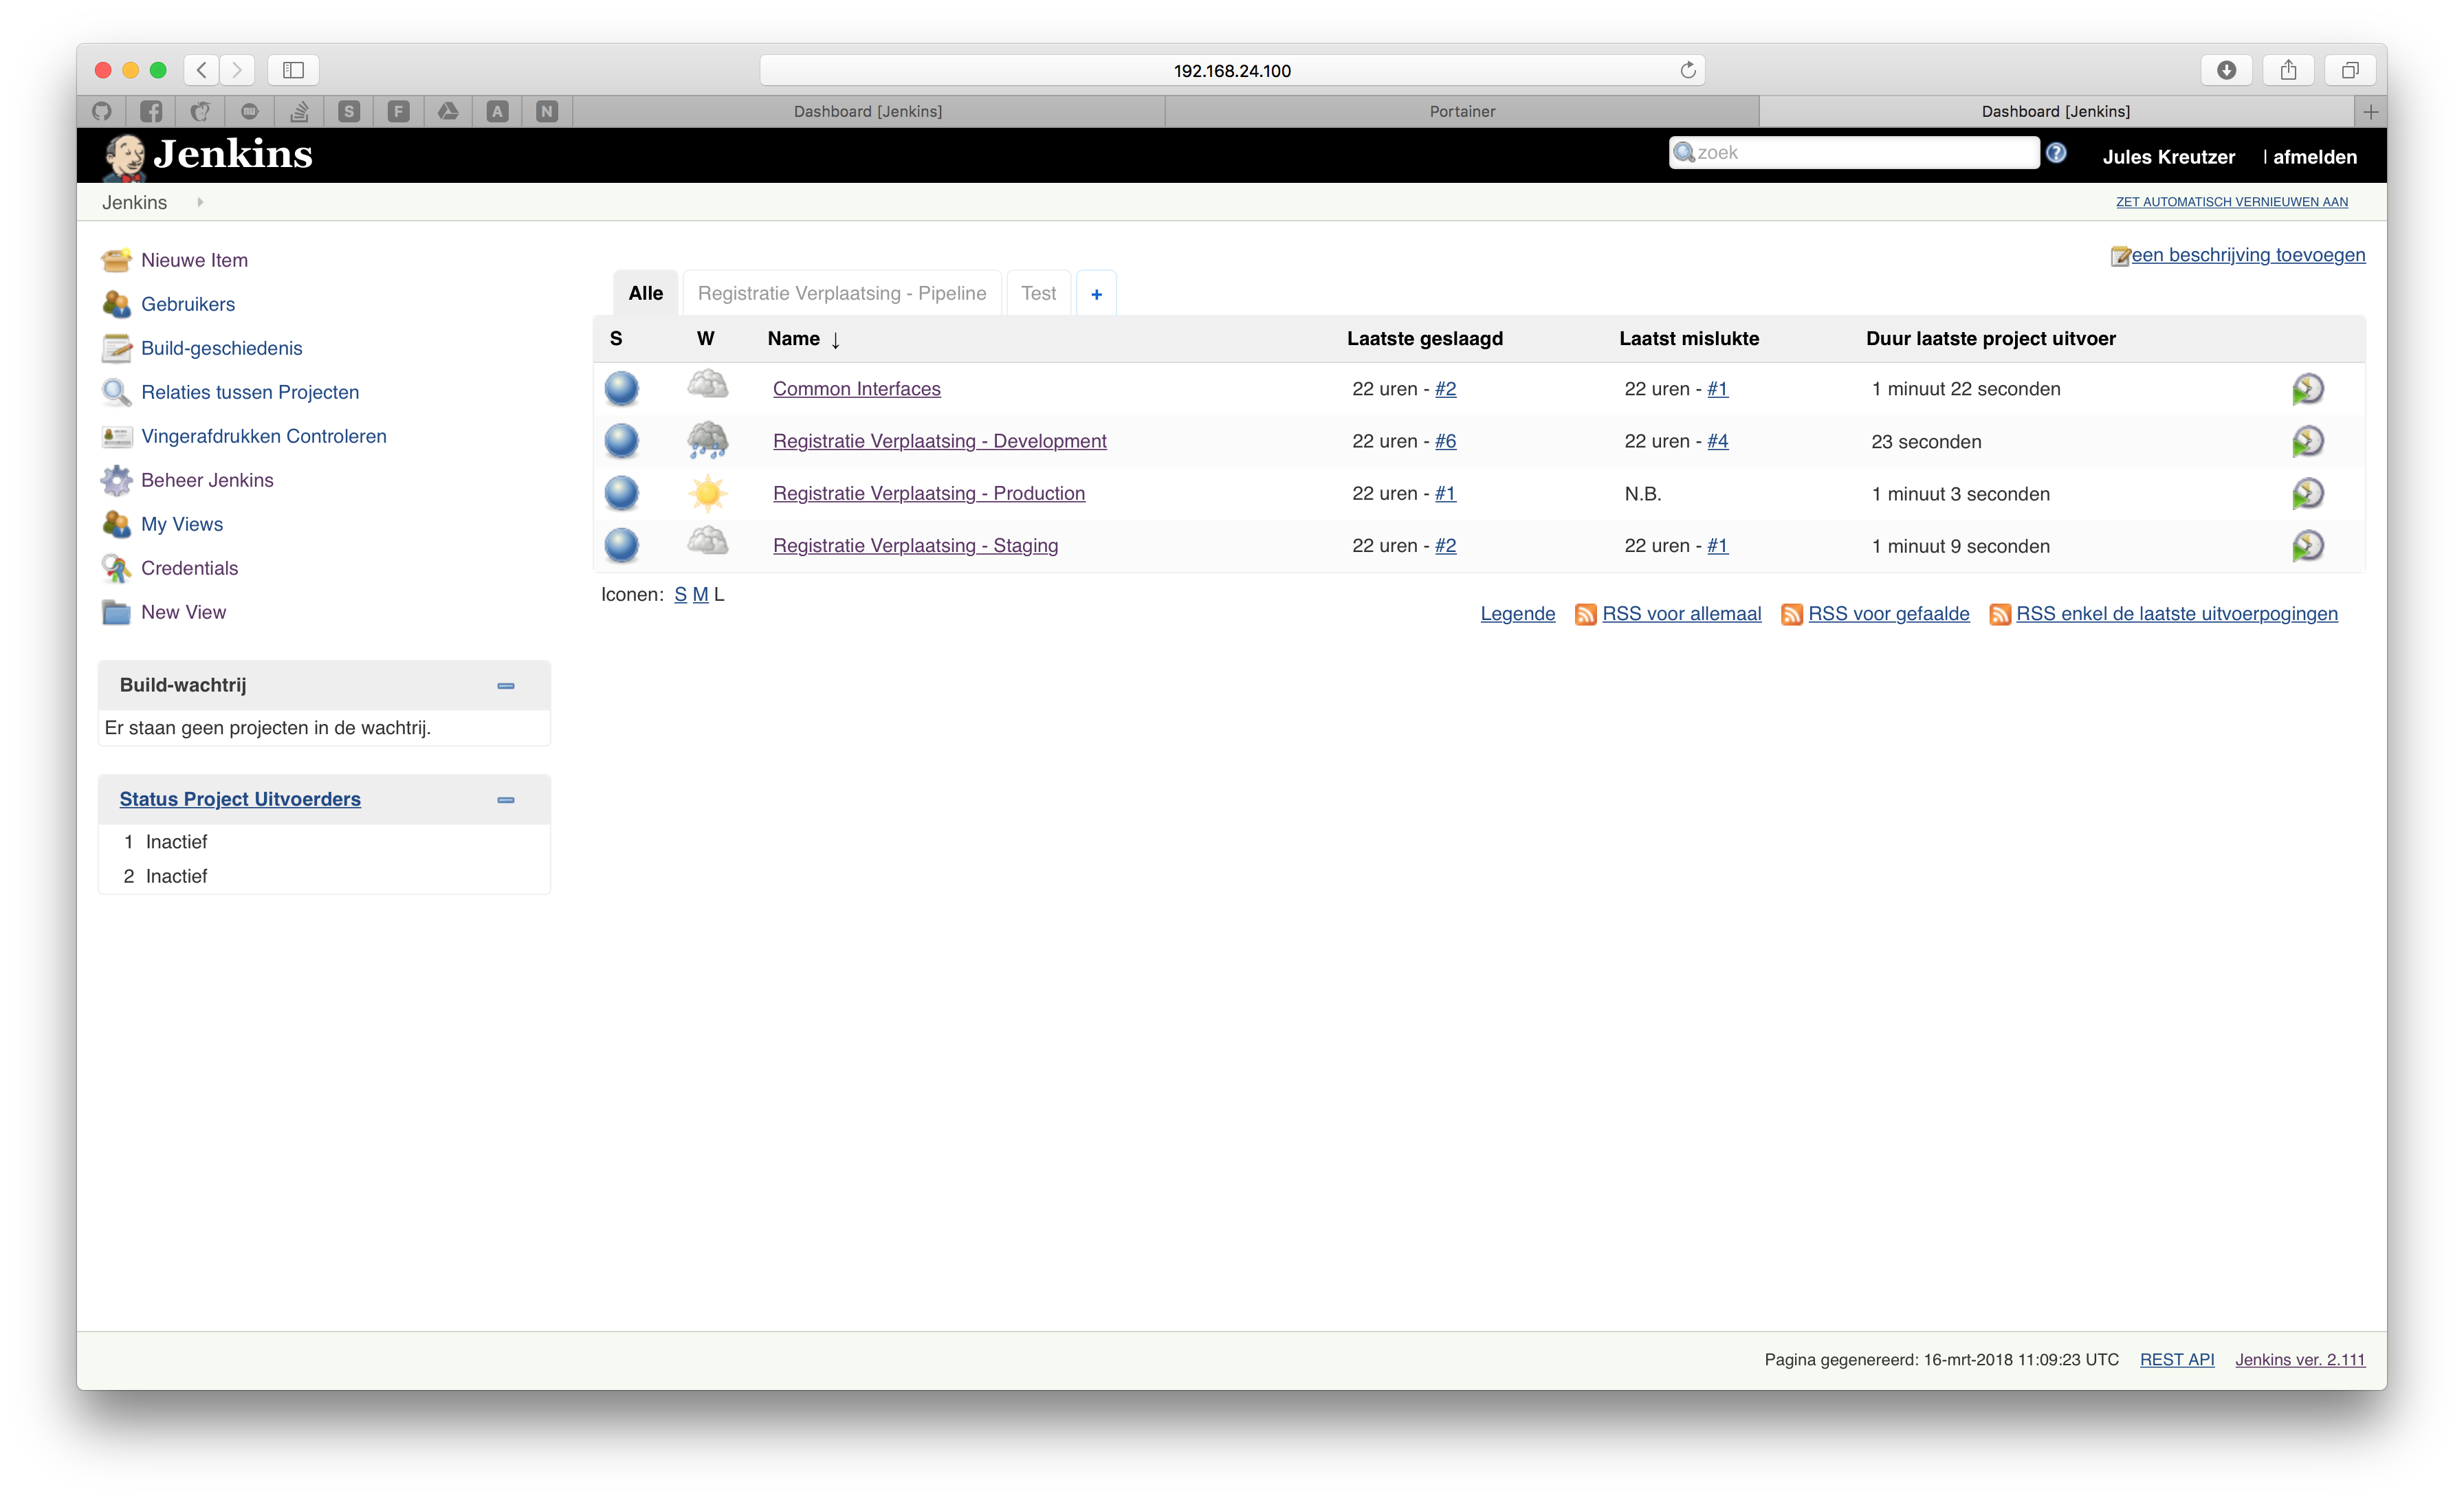
\includegraphics[width=0.95\textwidth]{img/JenkinsProjectOverview.png}
	\caption{Overzicht van de verschillende projecten binnen Jenkins voor een applicatie}
	\label{fig:JenkinsProjectOverview}
\end{figure}

\newpage
\subsection{Maven Settings}
De verschillende applicaties die ontwikkeld worden moeten met elkaar kunnen communiceren. Om de benodigde klassen hiervoor beschikbaar te krijgen in de verschillende applicaties hebben we ervoor gekozen om een nieuwe, "Common Interfaces", library te maken die beschikbaar is via Artifactory. 
Hiervoor moet een nieuwe repository toegevoegd worden en moet het gebruik van deze repository ook geauthorizeerd worden. Hiervoor moeten we de configuratie van maven aanpassen. Dit kunnen we doen in settings.xml of we kunnen een "global configuration file" in Jenkins aanmaken.

\begin{figure}[H]
	\centering
	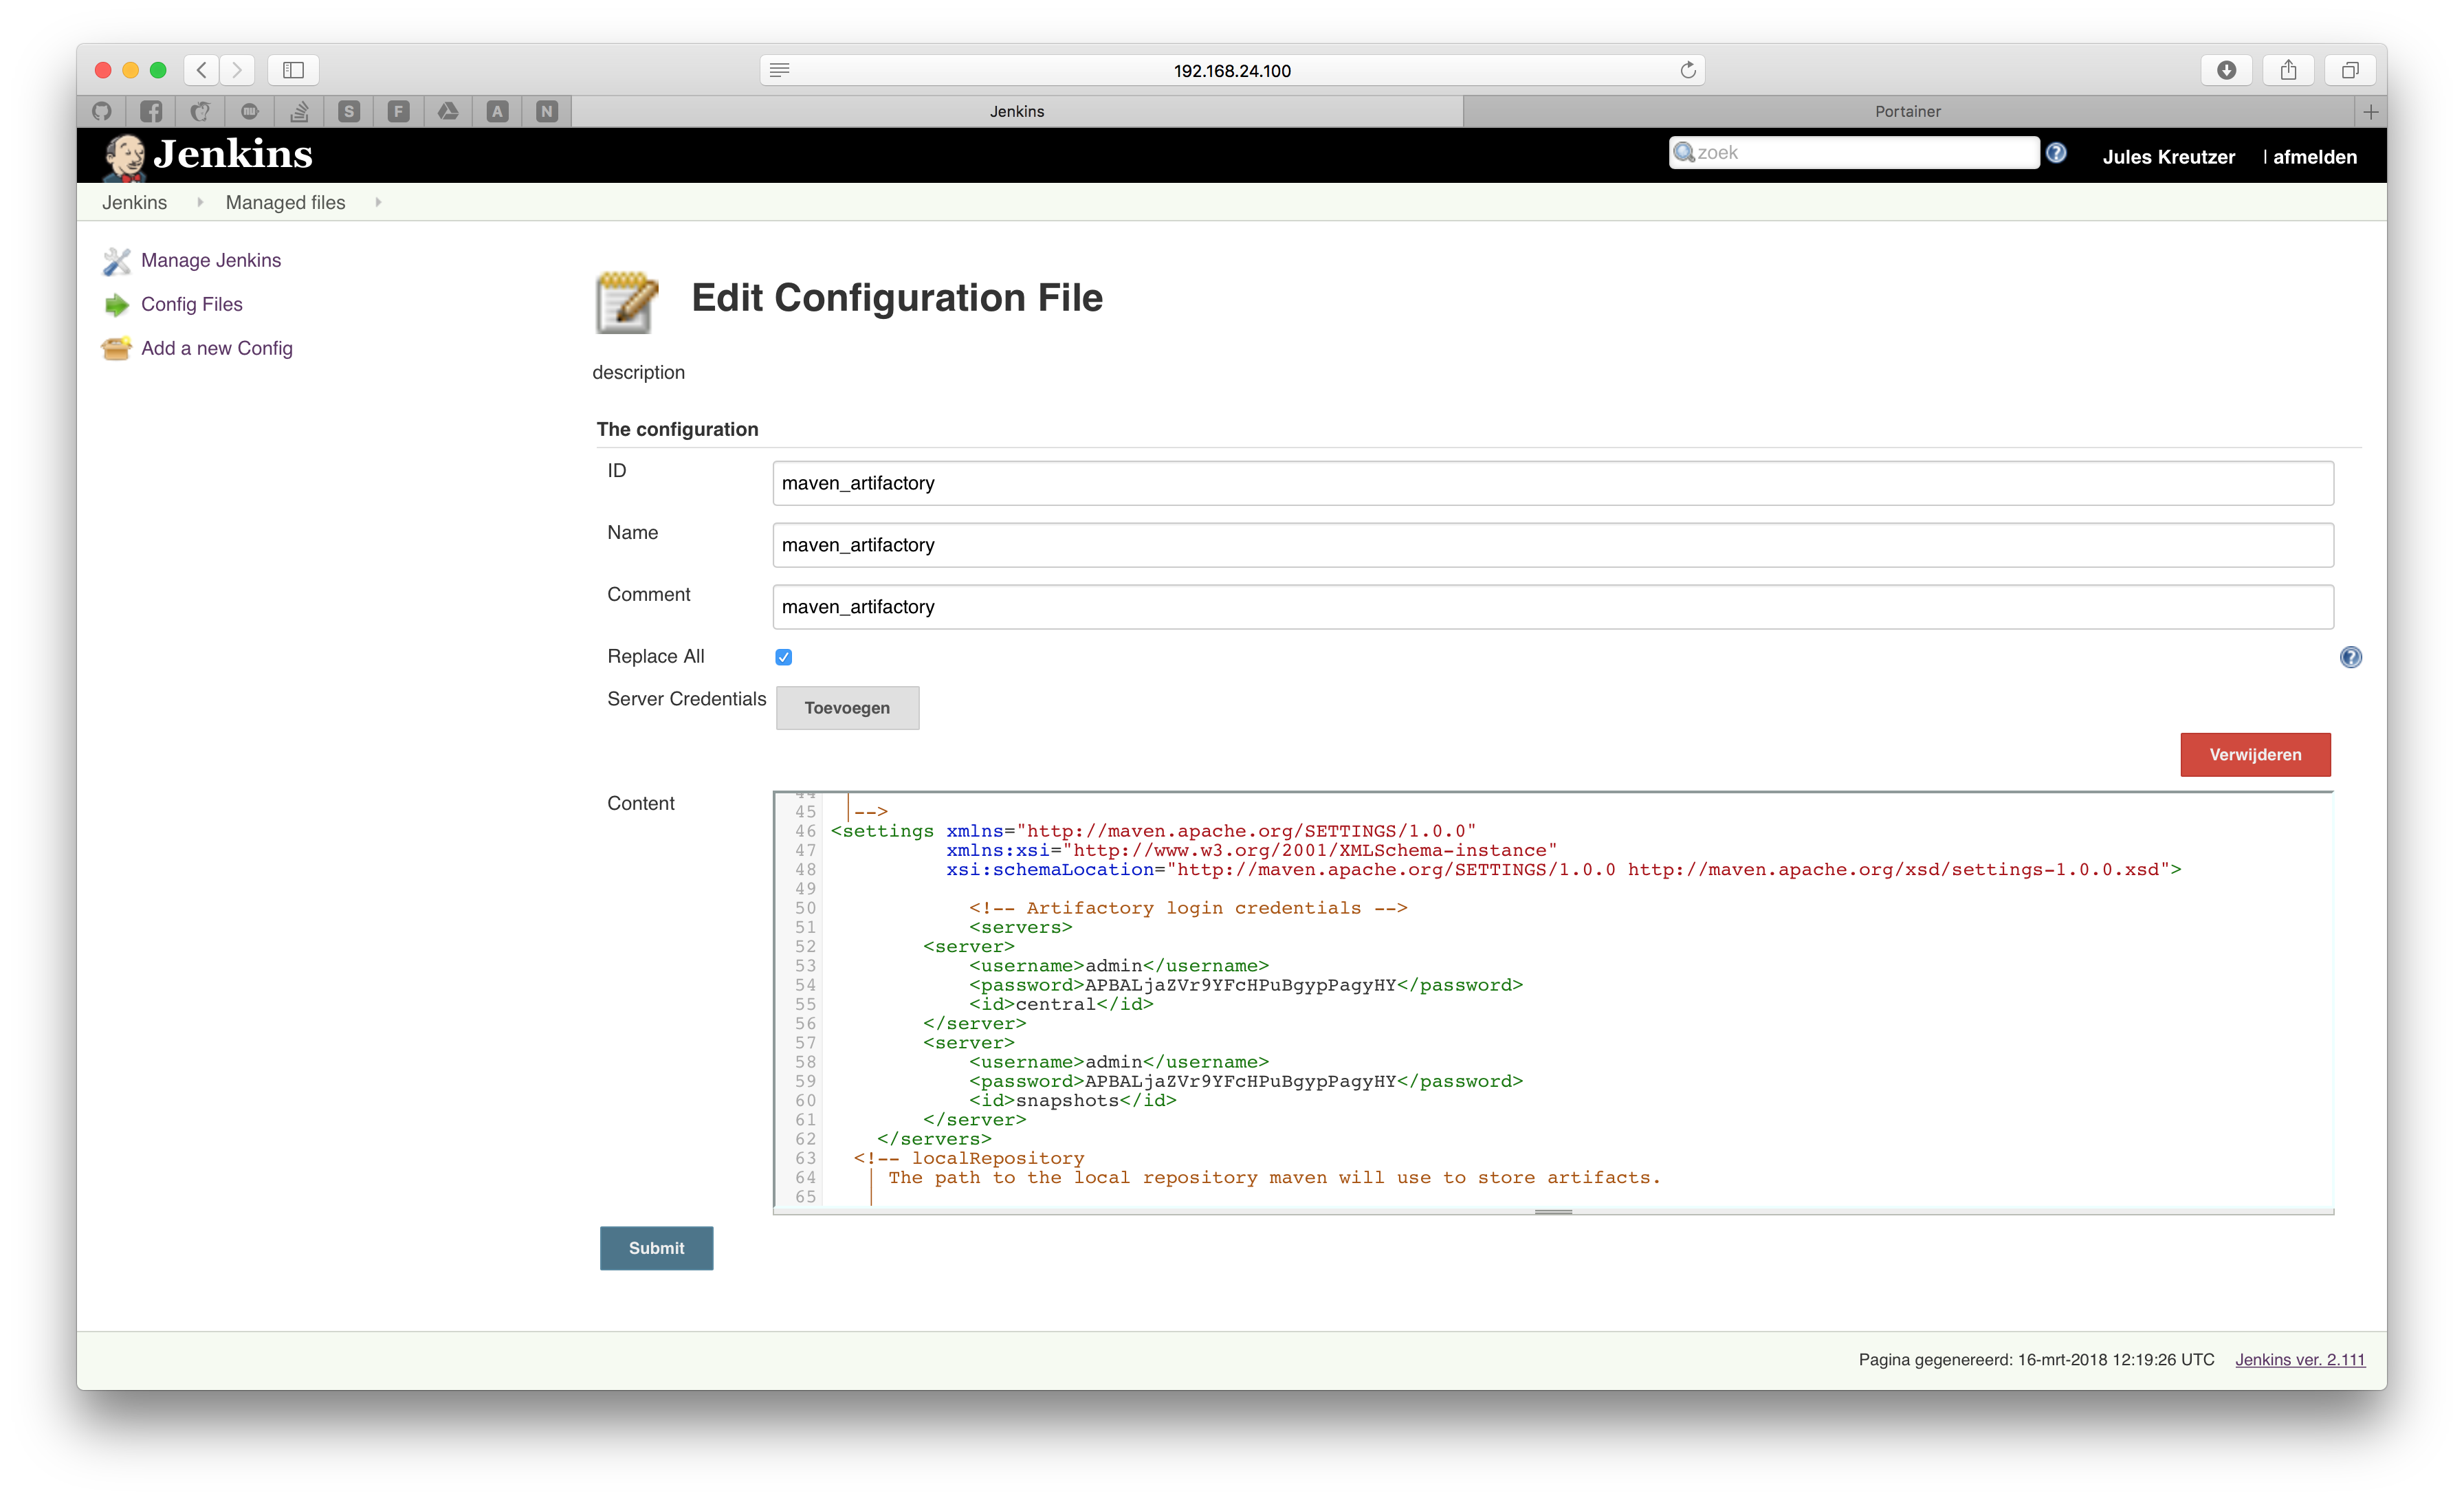
\includegraphics[width=0.95\textwidth]{img/MavenSettings.png}
	\caption{Global maven settings geconfigureerd met authorisatie voor Artifactory}
	\label{fig:MavenSettings}
\end{figure}
//TODO verwijzing naar configuratie van project
In bovenstaande afbeelding is zichtbaar hoe het nieuwe configuratie bestand voor de Maven settings eruit ziet. In hoofstuk XX wordt beschreven hoe deze configuratie gebruikt kan worden met een project

\subsection{Configuratie van Project}
Voor elke applicatie zijn er 3 verschillende projecten geconfigureerd. Deze projecten verschillen van elkaar in het uitvoeren van bepaalde automatische testen en de omgeving waarop de applicaties beschikbaar zijn. De verschillen in de configuratie worden, wanneer van toepassing, beschreven per hoofdstuk.
\newpage
\subsubsection{Bronbeheer}
Voor alle applicaties is be source code beschikbaar op Github. Voor het bouwen van de applicaties in Jenkins zal de sourcecode dan ook gepulled worden vanuit Github. Het verschil van de verschillende projecten is onder andere terug te vinden in welke branch gebruikt wordt voor het bouwen van de applicatie. Onderstaande lijst geeft een overzicht van de branch per project:

\begin{itemize}
	\setlength\itemsep{0em}
	\item Development - Development-branch
	\item Staging - Staging-branch
	\item Production - Master-branch
\end{itemize}

\subsubsection{Bouwactiveerders en Bouwomgeving}
De Development omgeving wordt automatisch gebouwd en getest door middel van unit tests bij elke commit en/of merge naar de Development branch op Github. 
\\
De Staging omgeving wordt één keer per week automatisch gebouwd, namelijk op dinsdag ochtend tussen 9:00 en 10:00. Het verschil met de development omgeving is dat bij het deployen van de Staging omgeving niet alleen de unit tests, maar ook bijbehorende integratie tests worden uitgevoerd.
\\ 
De Productie omgeving moet altijd handmatig gebouwd en deployed worden. Ook bij het bouwen van deze omgeving worden alle beschikbaar automatische tests uitgevoerd.

\begin{figure}[H]
	\centering
	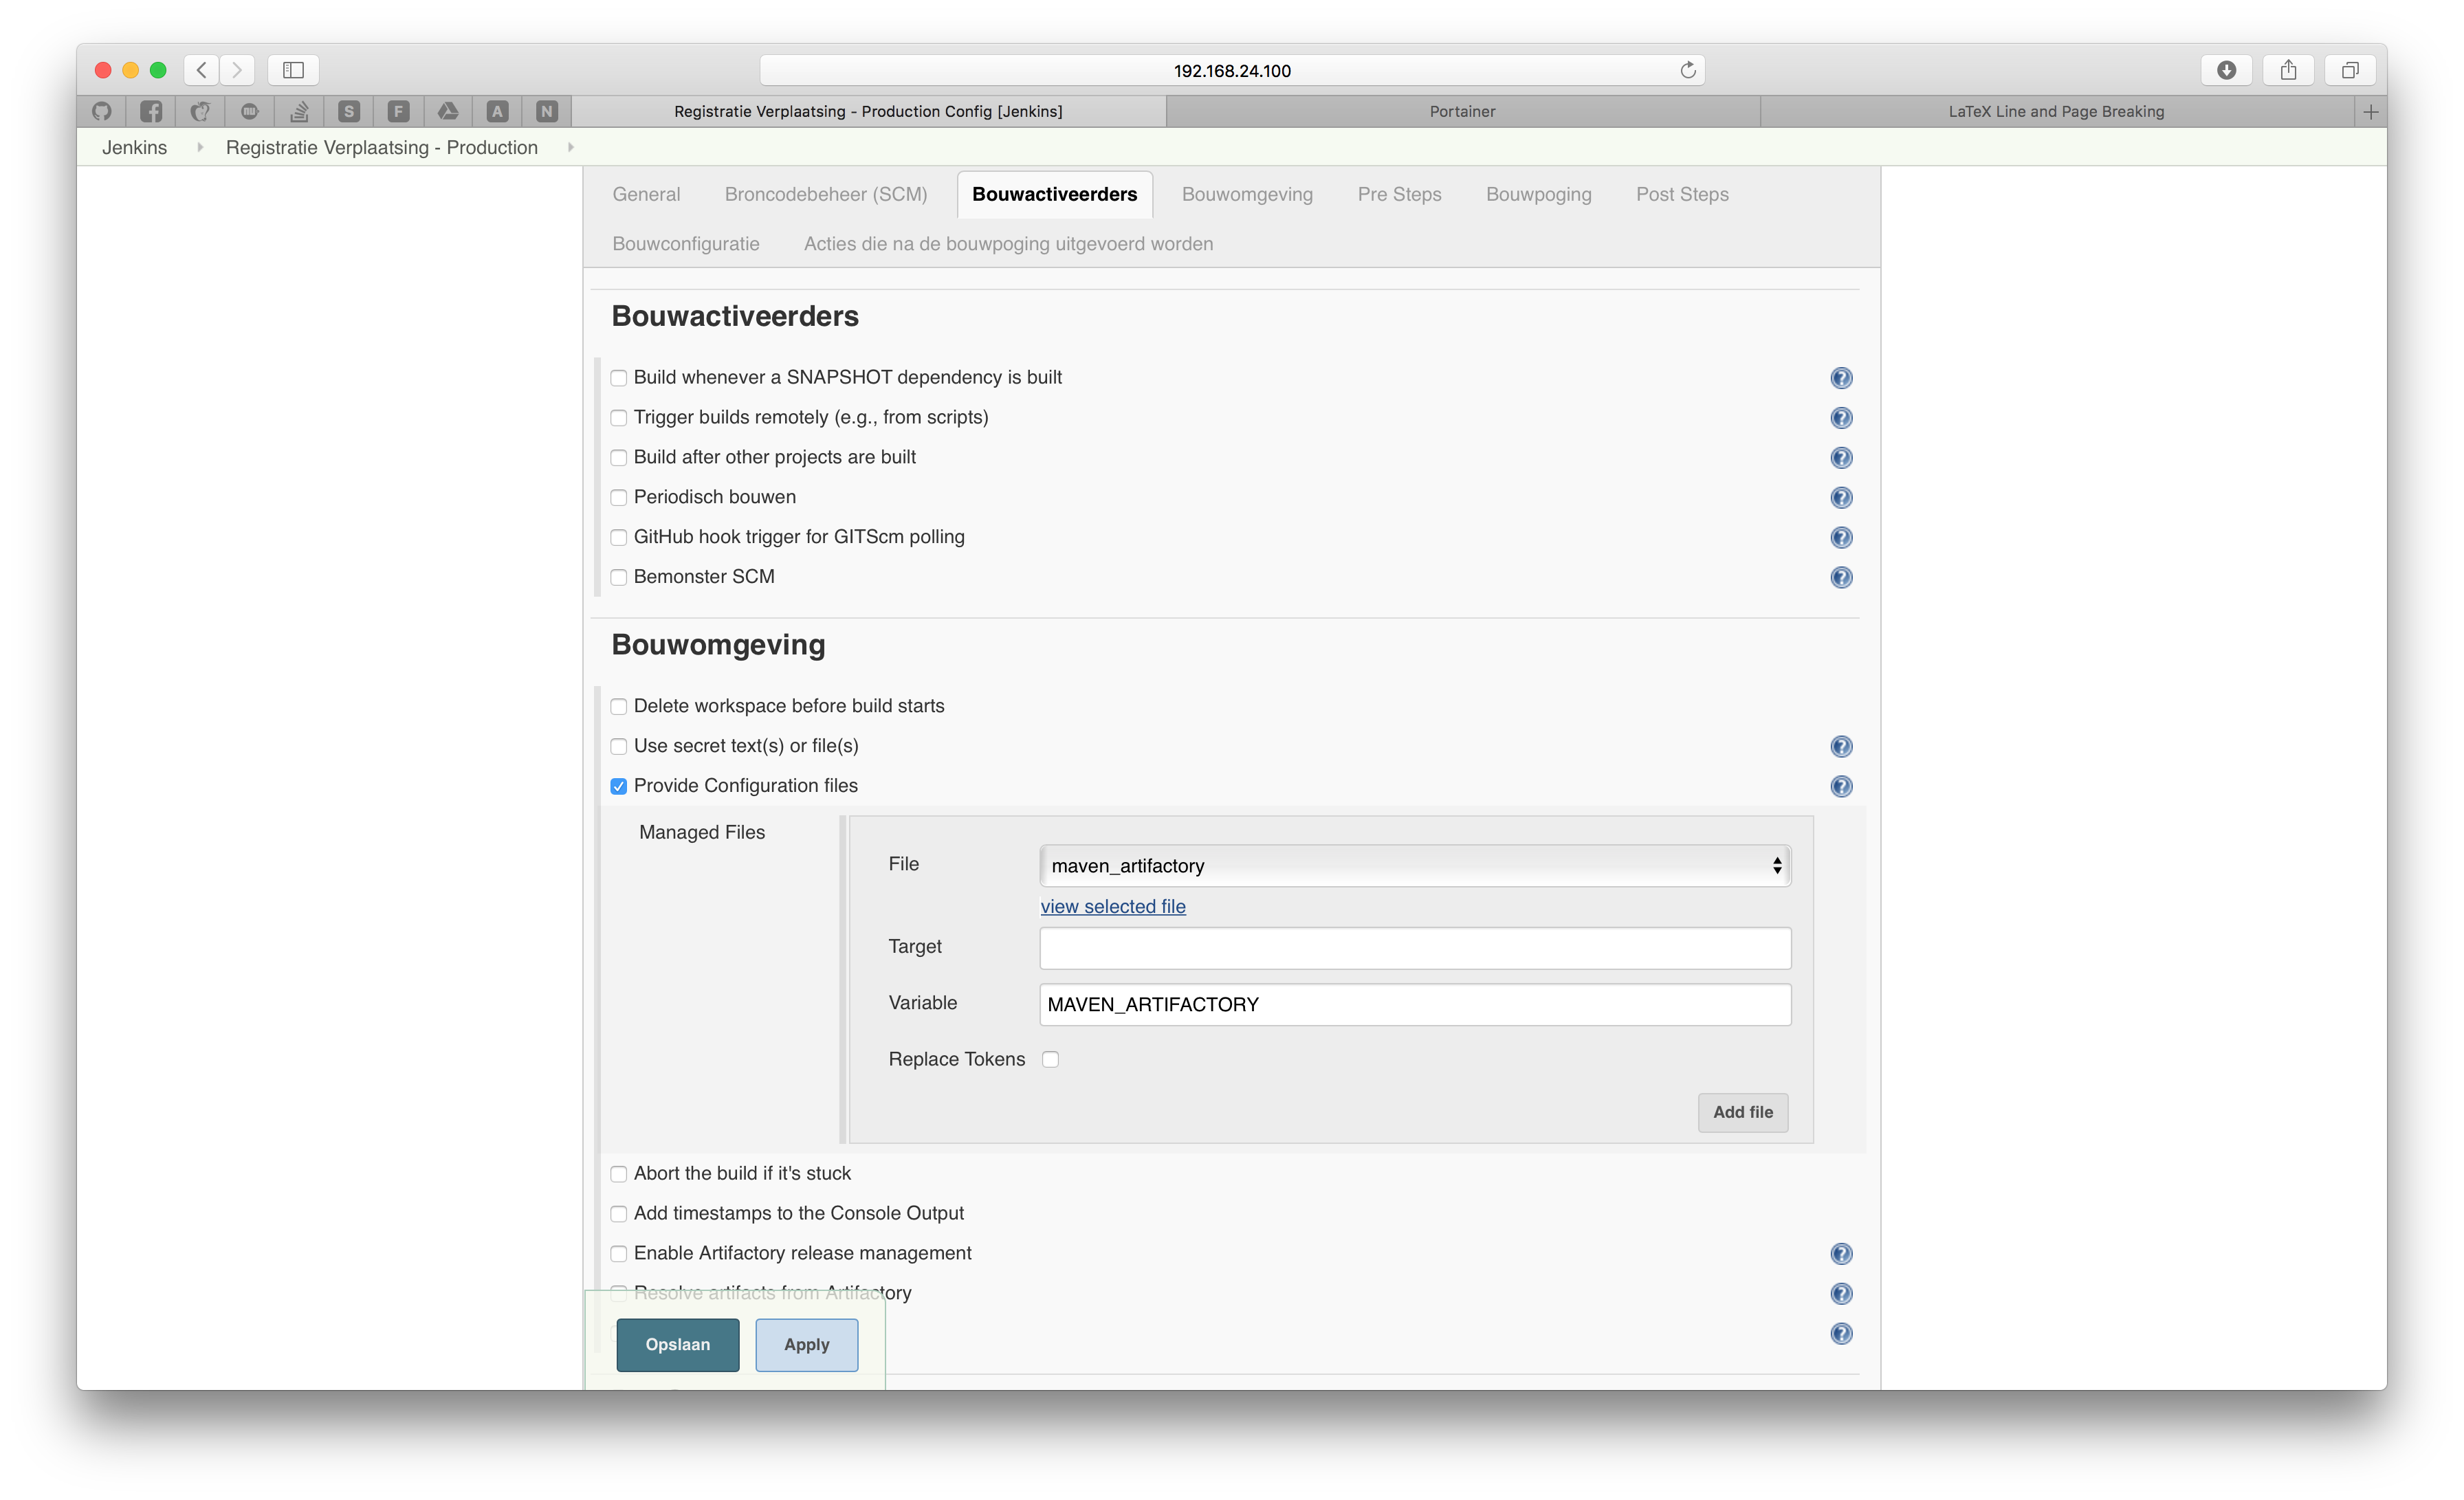
\includegraphics[width=0.95\textwidth]{img/JenkinsBouwactiveerdersBouwomgeving.png}
	\caption{Configuratie van Bouwactiveerders en Bouwomgeving in Jenkins}
	\label{fig:JenkinsBouwactiveerdersBouwomgeving}
\end{figure}

Zoals in de afbeelding hierboven te zien is wordt er een configuratie bestand toegevoegd aan de bouwomgeving. In deze configuratie file (maven\_artifactory) staat de authorizatie voor Artifactory beschreven zoals te zien is in figuur \ref{fig:MavenSettings}.

\newpage
\subsubsection{Bouwpoging}
Een belangrijk onderdeel voor het bouwen van de applicatie is het specificeren van verschillende zogenaamde "Maven goals". Dit zijn taken die worden uitgevoerd door Jenkins bij het bouwen van de applicatie.

Bij het bouwen van de productie omgeving worden onderstaande Maven goals gebruikt: 
\begin{lstlisting}
clean install package test 
		-P production
		-e sonar:sonar 
		-Dsonar.host.url=http://85.144.215.28:9001 
		-Dsonar.login=089ecbe71f30a12f9af77098b09921b83cf88786
\end{lstlisting}

Met bovenstaand commando wordt de working directory van het project eerst leeg gemaakt, de benodigde dependencies gedownload, de applicatie wordt verpakt zodat het kan worden uitgevoerd op een applicatie server en vervolgens worden de verschillende beschikbare automatische tests uitgevoerd.
\\
Voor het uitvoeren van de tests wordt het profiel "Production" gebruikt. Door middel van verschillende profielen kunnen we aangeven welke tests uitgevoerd moeten worden. De Development omgeving gebruikt bijvoorbeeld het profiel "Development" waarmee enkel unit tests worden uitgevoerd.
\\
Daarnaast worden verschillende Sonarqube gerelateerde parameters meegegeven. Dit zorgt ervoor dat er een analyse van de applicatie wordt gemaakt die na het bouwen van de applicatie kan worden geraadpleegd in Sonarqube.
\newpage
\subsubsection{Acties na bouwpoging}
Wanneer het bouwen van de applicatie geslaagd is, worden de gemaakte applicaties gedeployed en verstuurd naar Artifactory. Hierdoor kunnen we voor elke versie een geschiedenis bijhouden van de verschillende versies van de applicaties.
\\
Voor het deployen van de gebouwde applicatie op een applicatie server, maken we gebruik van de mapping die we in Portainer hebben opgezet zoals te zien is in figuur \ref{fig:JenkinsContainerDetails}.

Aan de hand van onderstaande code, wordt na het voltooien van de bouwpoging de applicatie verplaatst naar de "Autodeploy"\ folder binnen de container.
\begin{lstlisting}
cd target && mv *.war /autodeploy
\end{lstlisting}
Omdat de /autdeploy folder gemapped is naar de folder /opt/glassfish/autodeploy, is de applicatie ook beschikbaar op de host machine. Wat verder met deze applicatie wordt gedaan staat beschreven in hoofstuk 5: Applicatie Server.



\begin{figure}[H]
	\centering
	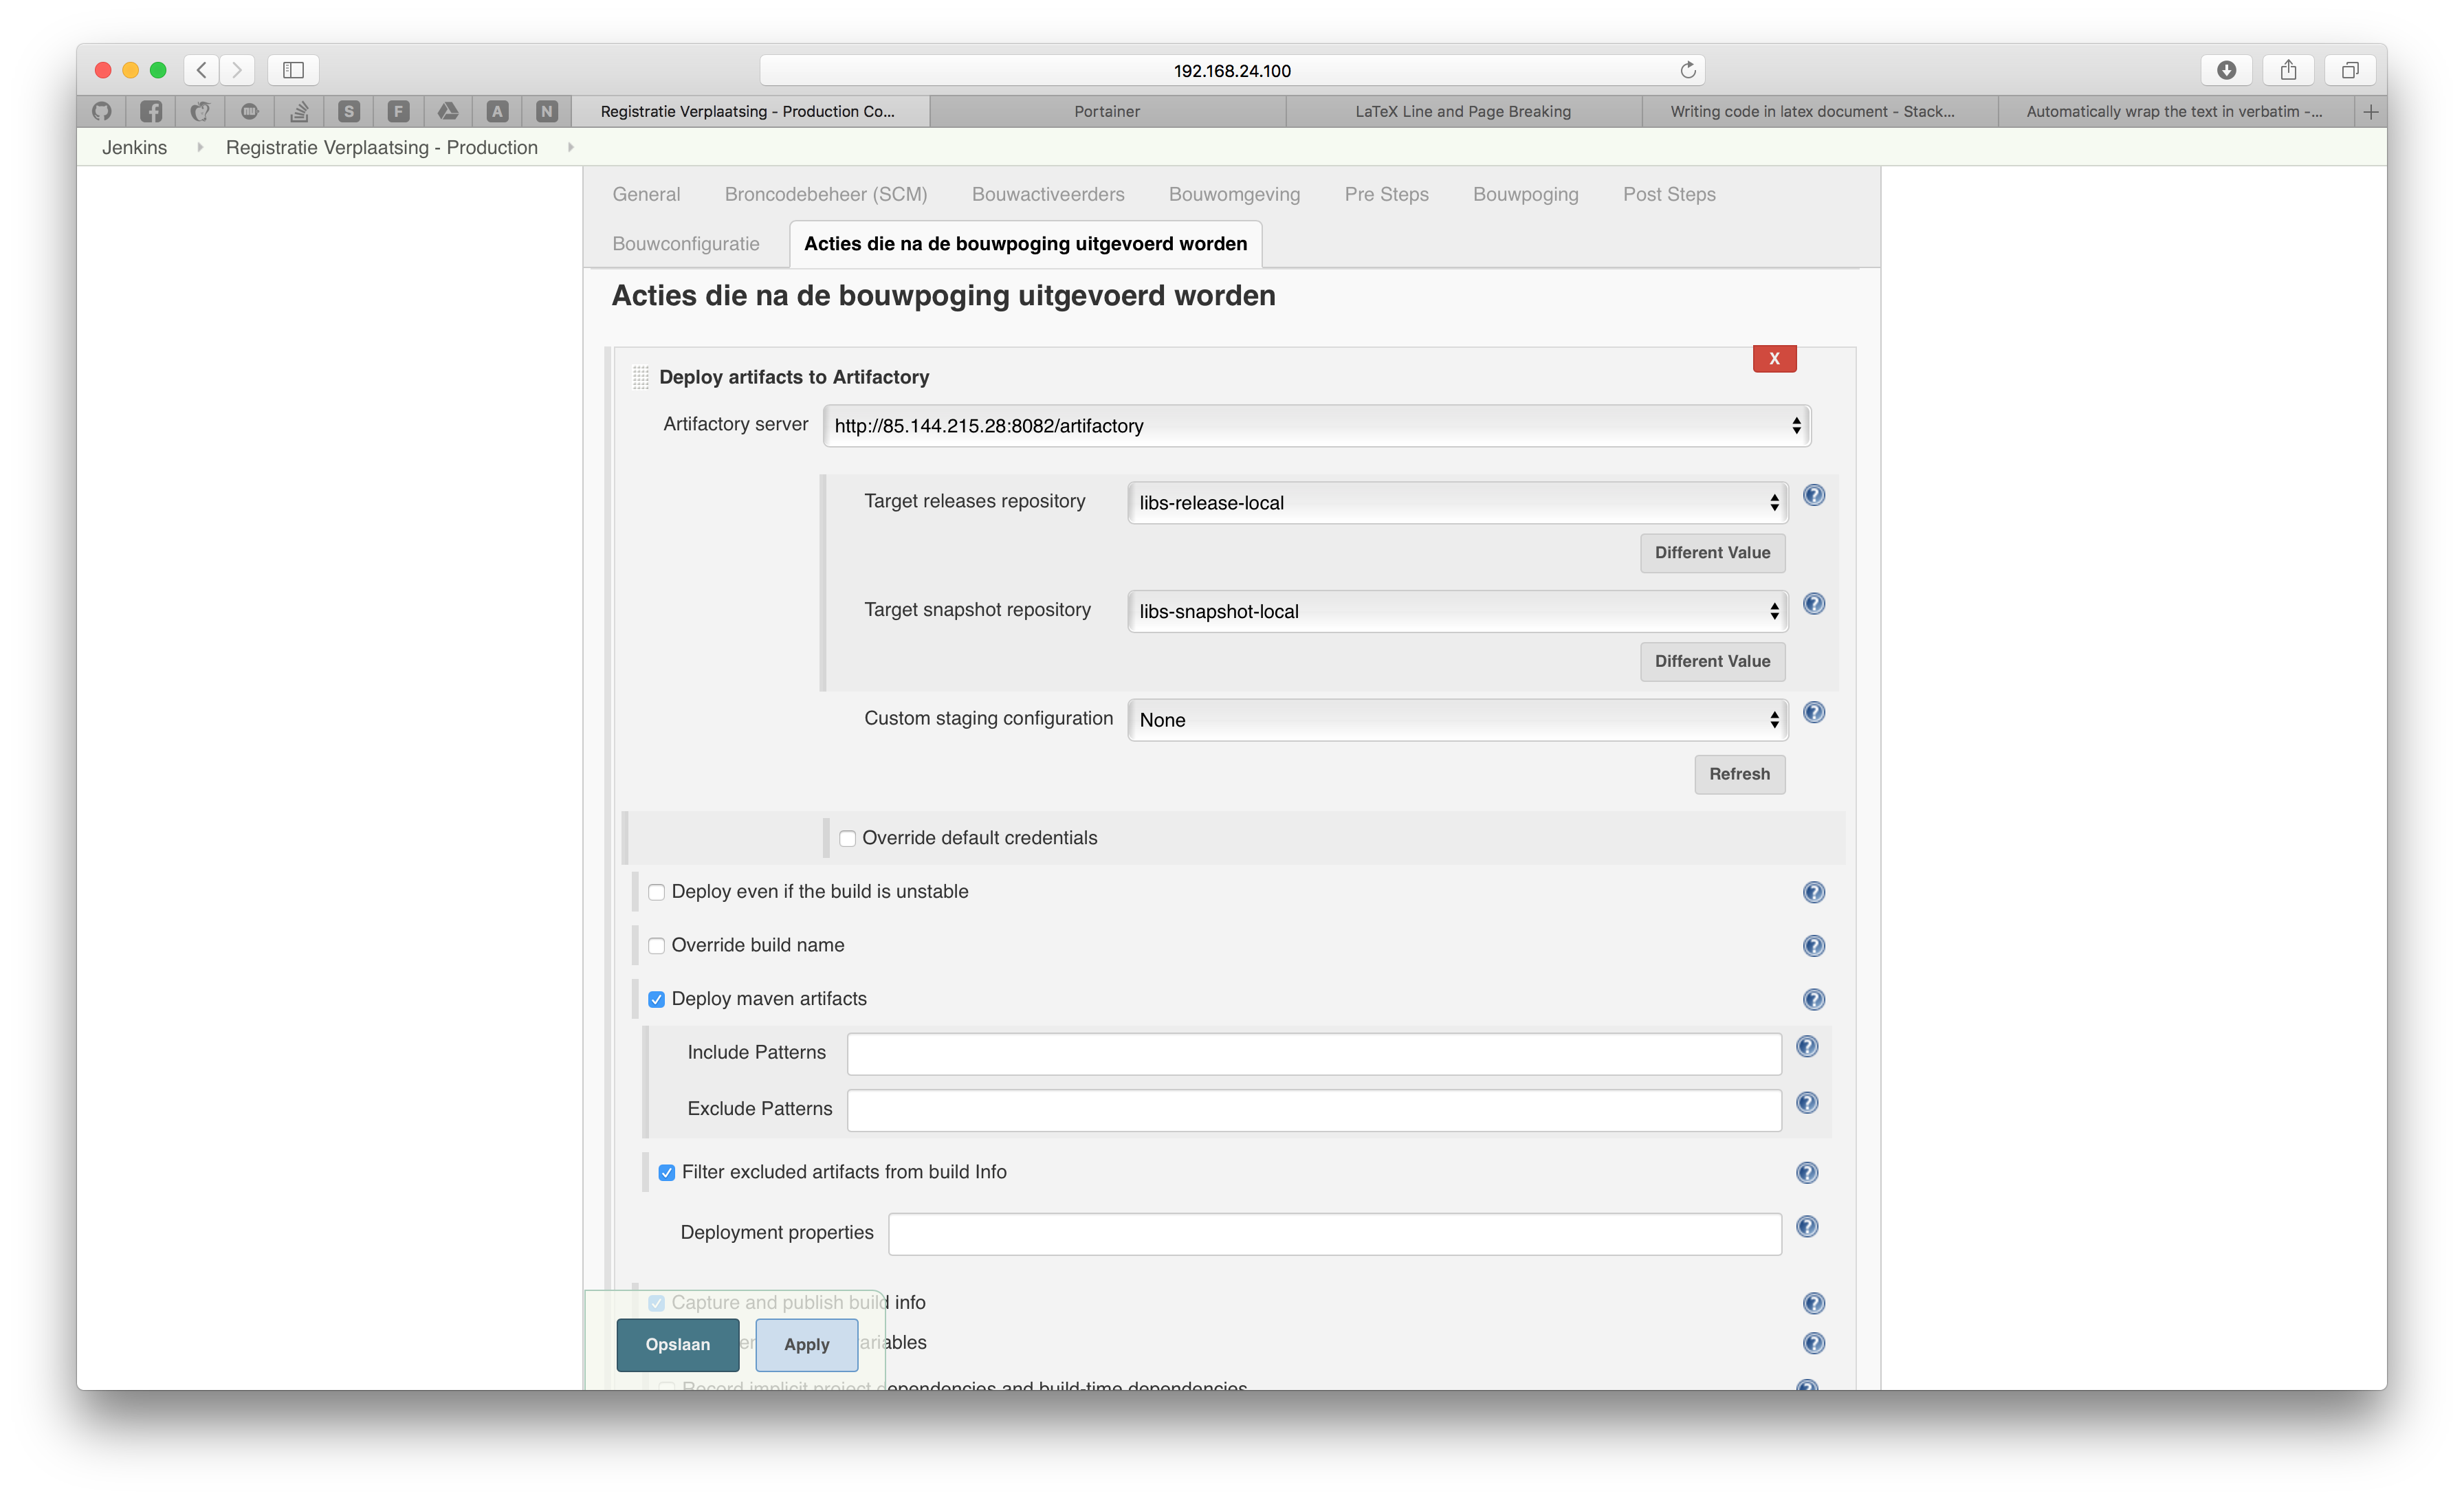
\includegraphics[width=0.95\textwidth]{img/ArtifactoryDeploy.png}
	\caption{Deployment configuratie voor Artifactory in Jenkins project}
	\label{fig:ArtifactoryDeploy}
\end{figure}